\documentclass[border=10pt]{standalone}
\usepackage{pgfplots}
\pgfplotsset{compat=1.18}

\begin{document}
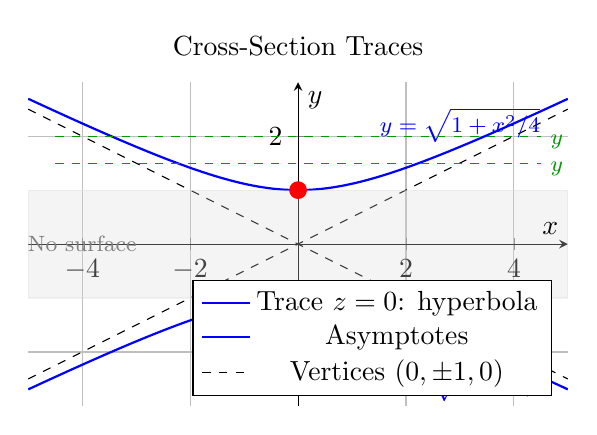
\begin{tikzpicture}
\begin{axis}[
    xlabel={$x$},
    ylabel={$y$},
    title={Cross-Section Traces},
    xmin=-5, xmax=5,
    ymin=-3, ymax=3,
    axis lines=center,
    grid=major,
    legend pos=south east,
    samples=100,
    axis equal image,
]
% Trace in xy-plane (z=0): y^2 - x^2/4 = 1 (upper branch)
\addplot[blue, thick, domain=-5:5] {sqrt(1 + x^2/4)};
\addplot[blue, thick, domain=-5:5] {-sqrt(1 + x^2/4)};
\addlegendentry{Trace $z=0$: hyperbola}

% Asymptotes
\addplot[black, dashed, thin, domain=-5:5] {x/2};
\addplot[black, dashed, thin, domain=-5:5] {-x/2};
\addlegendentry{Asymptotes}

% Vertices
\addplot[red, only marks, mark=*, mark size=3] coordinates {(0,1)};
\addplot[red, only marks, mark=*, mark size=3] coordinates {(0,-1)};
\addlegendentry{Vertices $(0,\pm 1, 0)$}

% Forbidden region
\addplot[gray!30, fill, opacity=0.3] coordinates {(-5,-1) (5,-1) (5,1) (-5,1) (-5,-1)};
\node[gray, font=\footnotesize] at (-4, 0) {No surface};

% Labels
\node[blue, font=\footnotesize] at (3, 2.2) {$y = \sqrt{1 + x^2/4}$};
\node[blue, font=\footnotesize] at (3, -2.6) {$y = -\sqrt{1 + x^2/4}$};

% Horizontal lines for circular cross-sections
\draw[dashed, green!60!black] (-4.5, 1.5) -- (4.5, 1.5);
\node[green!60!black, font=\footnotesize, anchor=west] at (4.5, 1.5) {$y=1.5$: circle $r=\sqrt{5}$};

\draw[dashed, green!60!black] (-4.5, 2) -- (4.5, 2);
\node[green!60!black, font=\footnotesize, anchor=west] at (4.5, 2) {$y=2$: circle $r=\sqrt{12}$};

\end{axis}
\end{tikzpicture}
\end{document}